% AI-assisted: OpenAI Codex, OpenAI. Exact model/release date unconfirmed.
% WORKING DRAFT. The entrant has not completed human modification or review.
\documentclass[UTF8,fontset=windows,zihao=-4,a4paper]{ctexart}
\usepackage[margin=2.5cm]{geometry}
\usepackage{amsmath,amssymb,booktabs,tabularx,longtable,array,graphicx,float}
\usepackage[unicode,hidelinks]{hyperref}
\usepackage{url}
\hypersetup{pdftitle={公开观测约束下的九龙交通数字孪生与治理仿真},pdfauthor={},pdfsubject={技术定稿，AI信息与参赛者复核待补}}
\setCJKmonofont{SimSun}
\urlstyle{same}
\setlength{\emergencystretch}{3em}
\setlength{\parindent}{2em}
\linespread{1.0}
\pagestyle{plain}
\ctexset{section={format=\centering\heiti\zihao{4}},subsection={format=\songti\zihao{-4}},subsubsection={format=\songti\zihao{-4}}}
\renewcommand{\arraystretch}{1.15}
\newcolumntype{Y}{>{\raggedright\arraybackslash}X}
\newcommand{\aicredit}{\par\noindent AI辅助说明：本节模型、程序、结果分析和图表由OpenAI Codex实质辅助，参赛者人工复核尚未完成，详见文后说明。\par}
\newcommand{\file}[1]{\texttt{\detokenize{#1}}}

\begin{document}
\begin{center}
{\heiti\zihao{3}公开观测约束下的九龙交通数字孪生与治理仿真}\par
\vspace{.6em}{\heiti 摘\quad 要}
\end{center}
以香港九龙公主道—加士居道周边为研究域，融合官方道路GIS、断面交通与历史归档，建立道路、合成车辆、设施、有效观测和事件共同组成的平行空间。采用非负最小二乘估计分时路径需求，通过SUMO微观仿真、占有率反馈和配对实验比较日常通行、拥堵治理与道路应急保障。

基准模型接入29个检测站，整理310548条30秒车道记录。58条候选路径仅受8个独立核心断面约束，矩阵秩为8，不能唯一识别真实OD。冻结15日先验后，17日及回溯未见的12、13日共36次跨日仿真均未通过项目自定的联合精度检查；12、13日08—09时的低速站窗分别为0/2、0/5复现。真实墙钟运行3600.007秒，60次HTTP请求全部成功，但12次需求决策均无合格约束并保持计划，证明本次工程运行成立，未证明精度提高。

治理A先核实道路空间占有率与E1断面时间占有率的单位差异，再建立带启停滞回的入口反馈。7种设计条件、3个新种子的21组同输入配对中，17组普通交通总经历量降低，4组增加，最差增加1.30\%；背景车辆21组均受损，成本增加14.34\%—43.77\%。等待保护候选虽减轻背景代价，却使最差总成本增加21.65\%—28.04\%，因此未替换原方案。

治理B设计1063.1米公共道路应急任务，保留车辆安全检查，增加稀疏让行与既有绿灯延长。12次任务均到达；入口治理A下耗时79—124.5秒，补充全绿参照为642.5—1934秒，但背景交通成本增加65.81\%—68.76\%。额外协同在原三种子及轻中重27次扩展中均未触发，未发现新增收益。全绿补充属于事后诊断，不作为独立现实验证。

系统将数据时间身份、未来计划、物理时刻、固定车辆对照和未完成成本纳入同一封装。结果支持公开数据下的仿真原型与条件性实验；真实转向、信号配时和初始排队仍缺，不能承诺现实精度、普遍治理收益或真实救援效果。

\noindent 关键词：非负最小二乘；微观仿真；占有率反馈；配对实验

\vspace{.5em}\noindent AI辅助及复核状态：本文涉及实质AI辅助；参赛者人工修改复核及工具版本信息尚待补齐。本版为技术定稿待复核版，不能直接声明全部提交条件已满足。
\newpage
\tableofcontents
\newpage
\section{问题重述}
研究区的城市干道存在主线通行、侧向汇入、分流和医院接近需求。断面计数能够描述局部交通，却不能直接给出完整OD、初始队列或真实车辆轨迹。B题要求以官方可靠GIS及实时提取数据为基础，在一个封装系统中建立平行空间和交通流仿真，回答三类情景的结构、数据、模型与效果问题。

问题一建立一般交通基准，并说明泛化能力；问题二在拥堵条件下构建治理A，比较治理前后交通效果；问题三增加应急管控、任务和保障协同，建立治理B，并与前项实验比较。三问共享数据与道路、车辆表示，但只有同网络、同输入、同事件和同评价时窗的实验才能直接计算治理收益。结果还须展示仿真步长与物理时间的对应。

\section{问题分析}
\subsection{问题一：从稀疏断面到可检查的平行空间}
完整OD和逐车实测轨迹不可得，直接把断面流量当出发需求会重复计数。本文选择有限候选路径上的非负最小二乘反演，将路径率作为带先验的估计，再生成身份固定的合成车辆。路网、观测、移动代理、事件和控制通过统一运行目录封装。有效性分别由数据质量、守恒、三指标误差和冻结后的异日验证判断，不以拟合残差代替仿真验证。

\subsection{问题二：控制是否只是转移等待}
入口控制可能降低主线排队，也可能把等待推到入口外。只比较已到达车辆或主线速度会漏掉代价。因此在相同外部车辆下比较同设施全绿与条件占有率反馈，并以固定时窗全体经历量为主指标，同时核算背景车辆、末期未完成和低速漏报。需求、转向和供给的设计压力条件用于检验结论对未知输入的依赖。

\subsection{问题三：任务完成与普通交通的共同约束}
应急方案既要检查任务是否完成，也要检查普通交通是否受损。模型将事件、任务出发和截止时刻固定，以无专门协同为同情景参照。换道请求必须符合空位、权限与后续路径条件；信号操作只延长当前已有绿灯。未完成任务在共同截止时刻保留经历量下界，避免只统计成功任务造成选择偏差。

\section{假设与适用范围}
\begin{enumerate}
\item 研究对象是选定片区的主走廊及相关支路。98条外部边用于普通与入口实验，125条用于应急；“全域”在本文中指已声明的研究域，并非整个香港交通系统。
\item GIS提供道路位置依据，OSM补充有向拓扑、车道及权限。两者不等同于逐连接实地核验；9个检测器映射保留复核标记，相关记录不进入需求约束。
\item 合成车辆的ID、时刻、路径、车型和速度因子由固定算法及种子生成。其身份与轨迹不是实测。候选路径反演不保证唯一真实OD，静态关联暂忽略路段传播时滞与蓄积。
\item 初始空网配合300秒预热，不假称预热已恢复真实队列。车型比例的反向借用、代表车长和驾驶参数均为显式假设。
\item 背景流900辆/小时、下游名义供给900辆/小时和拟议入口设施为设计条件。原有生成配时不代表现实信号；实际出流另行核算。
\item 应急事件与救援任务为设计实验。任务终点改为指定公共道路断面，不依赖医院专用救护门；不含出警准备、现场作业和医院交接。SUMO安全模式保留，不以零碰撞推出现实安全性。
\end{enumerate}

这些简化使系统可运行，但初始队列、真实转向与供给缺失仍会影响解释。因此后文既报告设计实验，也保留独立验证失败；二者不能互相替代。

\section{符号说明}
\noindent\begin{tabularx}{\textwidth}{lYl}
\toprule 符号 & 含义 & 单位\\\midrule
$G=(V,E)$ & 有向道路网络，节点及道路边集合 & —\\
$A_{dr}$ & 候选路径$r$是否经过检测断面$d$ & 0或1\\
$q_r,q_r^0$ & 路径小时率与均值先验 & 辆/小时\\
$y_d,\sigma_d$ & 有效时长扩展的断面小时率及条件标准差 & 辆/小时\\
$c_d$ & 观测窗口有效时长覆盖率 & 比例\\
$s,\Delta s,W$ & 仿真时刻、步长及预热时长 & 秒\\
$T_0,T_{\rm obs},T_{\rm recv}$ & 案例评价起点、观测末时刻及接收时刻 & UTC+8\\
$p_i,a_i,b_i$ & 车辆计划出发、实际入网及到达仿真时刻 & 秒\\
$L,H$ & 统一评价时窗起止 & 秒\\
$C$ & 时窗内全体普通车辆经历量 & 辆·小时\\
$o_k,r_k$ & 上一控制周期模拟占有率、下一周期名义放行率 & \%，辆/小时\\
$N_{\rm end}$ & 共同截止未完成车辆数，含未出发车辆 & 辆\\
\bottomrule
\end{tabularx}

\section{问题一：数据、平行空间与基准仿真}
\subsection{数据条件与实践背景：对应一1、一2}
\aicredit
道路地理依据来自香港运输署第二代道路网络\cite{gis}，提取片区中心线2545条。交通源采用运输署战略性及主要道路检测数据\cite{traffic}，原接口为\url{https://resource.data.one.gov.hk/td/traffic-detectors/rawSpeedVol-all.xml}，无需API密钥；历史版本由官方归档接口取得\cite{archive}。医院位置、地址及急症室属性来自医院管理局开放记录\cite{hospital}。OSM只补充仿真拓扑和通行属性，按其开放许可标明来源\cite{osm}。

\begin{table}[H]\centering
\caption{实际数据与未取得信息}\label{tab:data}
\begin{tabularx}{\textwidth}{lYY}\toprule
对象 & 已有数据及处理 & 未取得或不可推断内容\\\midrule
地理道路 & 官方矢量、OSM有向连接、车道及权限 & 每处连接及现实配时的现场核验\\
断面交通 & 29个站点；15—16日310548条车道30秒记录 & 区域完整OD、完整轨迹、连续无缺测观测\\
分时输入 & 5568个15分钟站窗，4727个合格 & 反演路径率不唯一，不是真实OD\\
车型 & 官方比例及显式借用；固定类型/速度因子 & 南向所有车型分布和个体驾驶参数\\
应急接入 & 官方伊利沙伯医院及急症室、公共道路路线 & 救护专用门、内部交接、本地交叉流量\\
实时状态 & 原HTTP响应、接收时刻、观测时期、SHA256 & 当前全域状态、分钟级无延迟保证\\\bottomrule
\end{tabularx}
\end{table}

15—16日有效覆盖约63.8\%和70.1\%。每30秒volume按该时段车辆数处理，小时率在完整有效时段上换算；m/s转km/h只针对SUMO输出。无效、缺测和真实零值分别保存，车型重叠合计类别不重复相加。来源及原件哈希随材料保存，表\ref{tab:data}中的未知量不得以估计值换名为实测。

对站点先要求预期所有车道同时有效，且计数、速度、占有率满足范围检查。评价采用15分钟窗口，有效覆盖至少60\%且最大连续缺口不超过180秒。设窗口有效时长$t_v$秒、有效计数和$n_v$，则小时率估计为
\begin{equation}\widehat y=3600n_v/t_v,\qquad c=t_v/900.\label{eq:rate}\end{equation}
式\eqref{eq:rate}隐含有效时段可代表整窗的条件。泊松计数条件下的误差带只描述抽样噪声，不涵盖非随机缺测、映射错误或交通非平稳性。速度按有效计数加权，占有率按有效时长与车道汇总；定义在处理脚本和输出列中固定。

\begin{figure}[!htbp]\centering
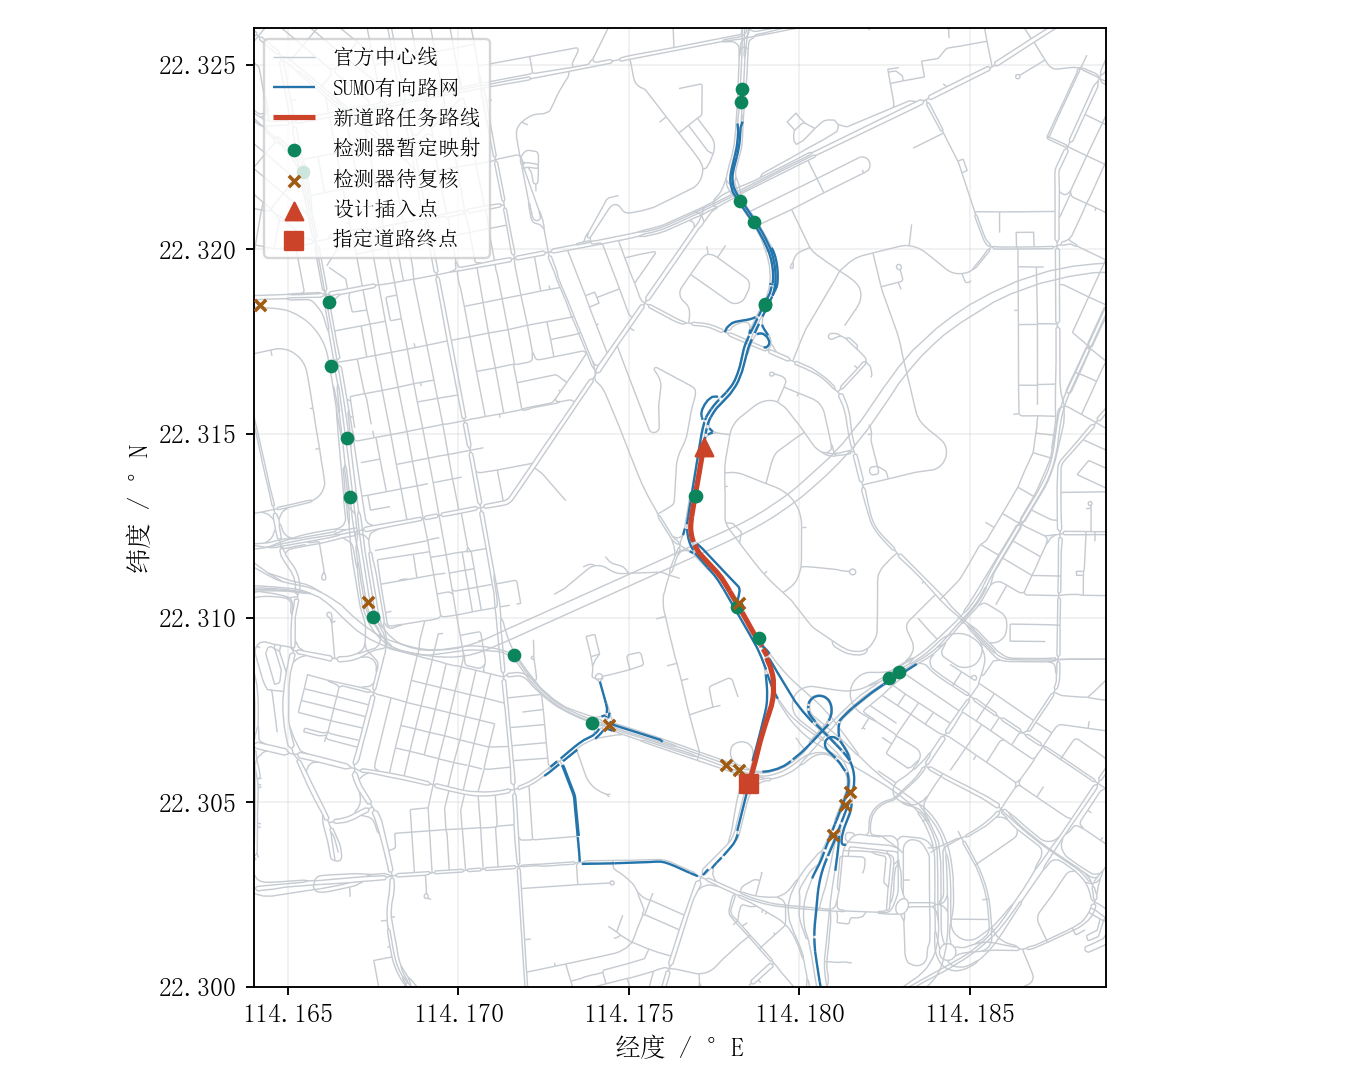
\includegraphics[width=.83\textwidth]{final_figures/study_area.png}
\caption{研究域、官方中心线、暂定检测器映射及指定公共道路应急路线。起终点是设计任务位置，不代表真实应急基地或停车许可。}
\label{fig:map}\end{figure}

图\ref{fig:map}中地理坐标为WGS84经纬度，仿真内部采用网络投影坐标。匹配综合距离、方向、路名、车道及高架/隧道层级，复核标记继续保留，不能由地图叠合自行认定正确。普通网继承生成信号，应急网增加与路线和信号相连道路，新增局部交通仍未知。

\subsection{孪生结构与封装：对应一1、一3}
平行空间状态定义为$S_s=(G,\mathcal A_s,\mathcal F_s,\mathcal O_s,\mathcal E_s)$：道路网络、移动代理、固定设施、带时间和质量标签的观测以及事件。移动代理保存合成ID、位置、速度、目的地和预计到达；固定代理包括道路、检测器、信号与指定公共道路终点。地理关系通过有向可达性、方向和距离约束表达。

程序将观测更新与仿真状态推进分别实现。前者检查有效性及可用时刻，后者在SUMO 1.27.1中按0.5秒推进并通过TraCI交互\cite{sumo,traci}。使用SUMO默认Krauss跟驰机制及明确的车型参数\cite{krauss}，不声称驾驶行为已本地标定。每个运行目录封装网络、车辆清单、配置、参数、事件、观测、输出和哈希；命令入口负责准备、运行、评价和离线回放，新增输入只影响尚未安排的未来车辆。

以赛题的状态更新思想记物理观测更新为$\delta$、符号映射为$Y$，系统采用
\begin{equation}
O_k=\delta(O_{k-1},I_k),\quad D_k=Y(O_k,G),\quad
S_{s+\Delta s}=F(S_s,u_s,D_k).
\label{eq:state}
\end{equation}
$I_k$只包含当时已取得且质量合格的观测，$u_s$是控制和事件。式\eqref{eq:state}区分观测更新与仿真推进：观测约束聚合需求，车辆按跟驰和路权与邻车交互，入口反馈随局部状态调整，形成复杂适应系统的局部交互机制；拓扑保证有向可达，方向和距离保证几何映射。GIS提供空间依据，数字孪生思想提供状态和时间对应，而非宣称完整复制了物理世界。

本项目只有断面聚合观测，未建立真实车辆到数字个体的一对一身份映射。现实数据进入模型，控制建议在仿真中执行；没有向现实信号机下发指令。因此当前闭环范围是“观测—计划—模拟—评估”的系统原型。

\subsection{非唯一需求估计与固定合成车辆}
58条候选边界路径的计数约束少于未知路径率。设$A$为断面—路径关联矩阵，以合格且无复核标记的断面为约束，求解
\begin{equation}
\min_{q\geq0}\ \|W_d(Aq-y)\|_2^2+0.2^2\|q-q^0\|_2^2
+0.15^2\|q-q^{\rm prev}\|_2^2+\lambda_e^2\|Bq\|_2^2.
\label{eq:inverse}
\end{equation}
其中$W_{d,dd}=500/\max(100,\sigma_d)$，$B$按缺少直接证据的外部入口汇总路径率；治理实验取$\lambda_e=0.5$，用于限制无支撑的外部注入，并非断言入口真实为零。首窗不使用前窗项，无合格约束时保持先验。式\eqref{eq:inverse}通过SciPy的有界线性最小二乘求解器实现\cite{scipy}。关联模型忽略传播时滞与蓄积，因此静态拟合误差不能代替微观仿真误差。

在声明的8个独立核心断面上，$A$有58列、秩为8，零空间维数为50。数值构造得到不同的非负路径率$q$与$q'$满足$Aq=Aq'$，故即使静态计数完全相同，也不能证明OD唯一。正则项只是从可行解中选择有先验约束的代表解，不会新增真实观测。对此保留矩阵、替代解及哈希证据。

各路径累计取整的生成数量与连续期望差小于1；分层出发不越时间区间。车辆ID、计划出发、路径、车型、车长及速度因子在运行控制前固定。相同种子的不同治理方案复用完全相同清单。随机驾驶扰动仍可能在不同状态下分岔，故报告多个种子的配对结果，而非仅一条优选轨迹。

路网早期人工终点使部分直行车辆消失，后修复两类主线终点共12条路径的续接，保持明确侧出口。修复后的98边版本用于后续入口实验，旧失败网络与结果保留，不能把实现缺陷归因于真实交通机理。

\subsection{实时提取、时效与未来计划}
每条观测保留观测起止、实际HTTP接收或历史归档发布时间代理、决策时刻及质量。真实采集的年龄为$T_{\rm recv}-T_{\rm obs}$；早期接口检查约5.6—7.6分钟，因而“实时提取”不等于源数据无延迟。历史归档发布时间不冒充本机当年接收时刻。

滚动计划每300秒执行一次，只用决策时刻之前已可用的数据；回看900秒，覆盖至少80\%，最近观测年龄不超过600秒。约束不足或断流时保持上一计划，不把缺测当零需求。有效时重新求解式\eqref{eq:inverse}，各路径变化限制在$0.25\max(q^{\rm prev},q^0,10)$之内，只生成未来车辆，已发车辆不回改。


早期16分钟正常与6分钟预设断流运行核实了无约束保持和未来计划更新。随后另做一小时真实墙钟实验，实际3600.007秒、仿真3600秒，保存61帧；60次HTTP全部成功，取得40个不同响应，源延迟286—461秒。12次需求决策均因没有合格约束而保持计划，没有观测驱动的需求改变量，不能据此声称精度提高。

\begin{figure}[H]\centering
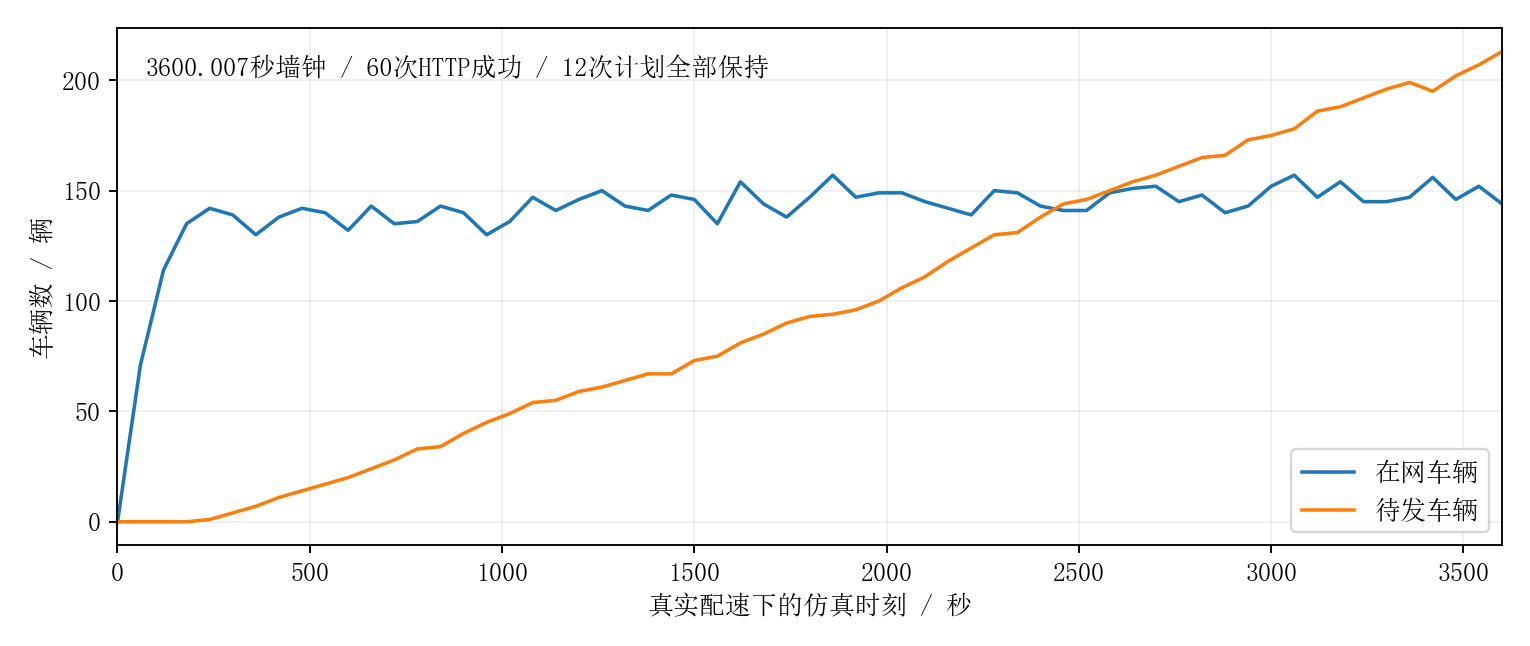
\includegraphics[width=.94\textwidth]{final_figures/live_hour.png}
\caption{一小时实际墙钟运行的系统输出。12次计划全部保持，曲线不代表已通过精度验证。}
\label{fig:live}\end{figure}
图\ref{fig:live}对应计划4827辆、到达4468辆、在网144辆、待发213辆、已加载尚未尝试2辆，故未完成359辆且守恒差为零。保存采样点最大滞后0.0041秒，不是所有仿真步的最坏滞后。此次零瞬移、零碰撞仅支持本次工程核算，不能外推全天候稳定性。

另接通4个官方视频统计镜头\cite{aivas}，240次成功HTTP得到900行、去重后275个统计时期。142条正流量有效、97条合法零流量的速度无定义、36条未来时间记录被排除。首请求至末接收3557秒且约130秒间歇采样，不等于连续一小时车流。15段几何核对未满足预定的单边接入条件，故未强行同化到原模型。官方信号设施图层\cite{tad}只给设施位置，医院公众导览\cite{hospitalmap}也不能补出实际配时或救护专用入口。

\subsection{物理时间、仿真步长与输出解释：对应一3}
每例以声明的评价起点$T_0$与预热$W=300$秒建立
\begin{equation}
T_{\rm case}(s)=T_0+(s-W),\qquad \Delta s=0.5\ {\rm s}.
\label{eq:clock}
\end{equation}
治理及应急案例$T_0$为2026-10-15 08:00、UTC+8，故$s=0$对应07:55，$s=2400$对应08:35。历史实验按此时间解释，不要求一秒计算耗时等于一秒物理时间。真实配速模式另以单调墙钟约束仿真推进，采集接收时间单独记录，不能把历史归档发布时间写成实际HTTP接收时刻。后文图\ref{fig:physical}直接展示时钟对应及车辆状态。

\subsection{多日验证与泛化边界：对应一4}
对合格同站同时窗计算流量WMAPE、速度和占有率MAE：
\begin{equation}
E_q=100\frac{\sum_j|\widehat q_j-q_j|}{\sum_jq_j},\quad
E_v=\frac1m\sum_j|\widehat v_j-v_j|,\quad
E_o=\frac1m\sum_j|\widehat o_j-o_j|.
\label{eq:errors}\end{equation}
并列低速复现/漏报/错报、未发、未完成、瞬移、碰撞和守恒。项目预设检查线为$E_q\le15\%$、$E_v\le5$\,km/h、$E_o\le5$个百分点；有低速时召回至少80\%、错报不超过10\%，另要求可比核心站窗至少50\%、无模拟速度缺失与异常守恒。该检查线不是赛题或当地行业标准。


15日先验、算法、时段及检查线冻结后，在17日开展普通/08—09时段、先验/滚动两种输入、三个新种子共12次验证；随后对12、13日各做同样12次。17日是周六，12、13、15日为工作日；12、13日早于训练日，称为回溯未见日期，不能写成未来预测。各日只仿真08—09和11:15—12，整日观测质量不等于整日仿真。

\begin{table}[H]\centering
\caption{跨日三种子均值；每行3次联合检查均未通过}\label{tab:holdout}
\begin{tabularx}{\textwidth}{lYlrrr}\toprule
日期 & 时段 & 输入 & 流量\% & 速度km/h & E1占有率pp\\\midrule
12日 & 普通 & 先验 & 6.36 & 6.09 & 1.61\\
12日 & 普通 & 滚动 & 9.00 & 5.96 & 1.45\\
12日 & 08—09 & 先验 & 13.02 & 13.34 & 3.67\\
12日 & 08—09 & 滚动 & 15.34 & 13.34 & 3.54\\
13日 & 普通 & 先验 & 8.49 & 6.14 & 1.50\\
13日 & 普通 & 滚动 & 10.32 & 6.09 & 1.36\\
13日 & 08—09 & 先验 & 15.90 & 16.20 & 5.64\\
13日 & 08—09 & 滚动 & 16.84 & 16.12 & 4.97\\
17日 & 普通 & 先验 & 10.71 & 9.89 & 2.65\\
17日 & 普通 & 滚动 & 10.98 & 9.84 & 2.67\\
17日 & 08—09 & 先验 & 25.22 & 7.07 & 3.04\\
17日 & 08—09 & 滚动 & 25.99 & 6.92 & 2.56\\\bottomrule
\end{tabularx}\end{table}
\begin{figure}[H]\centering
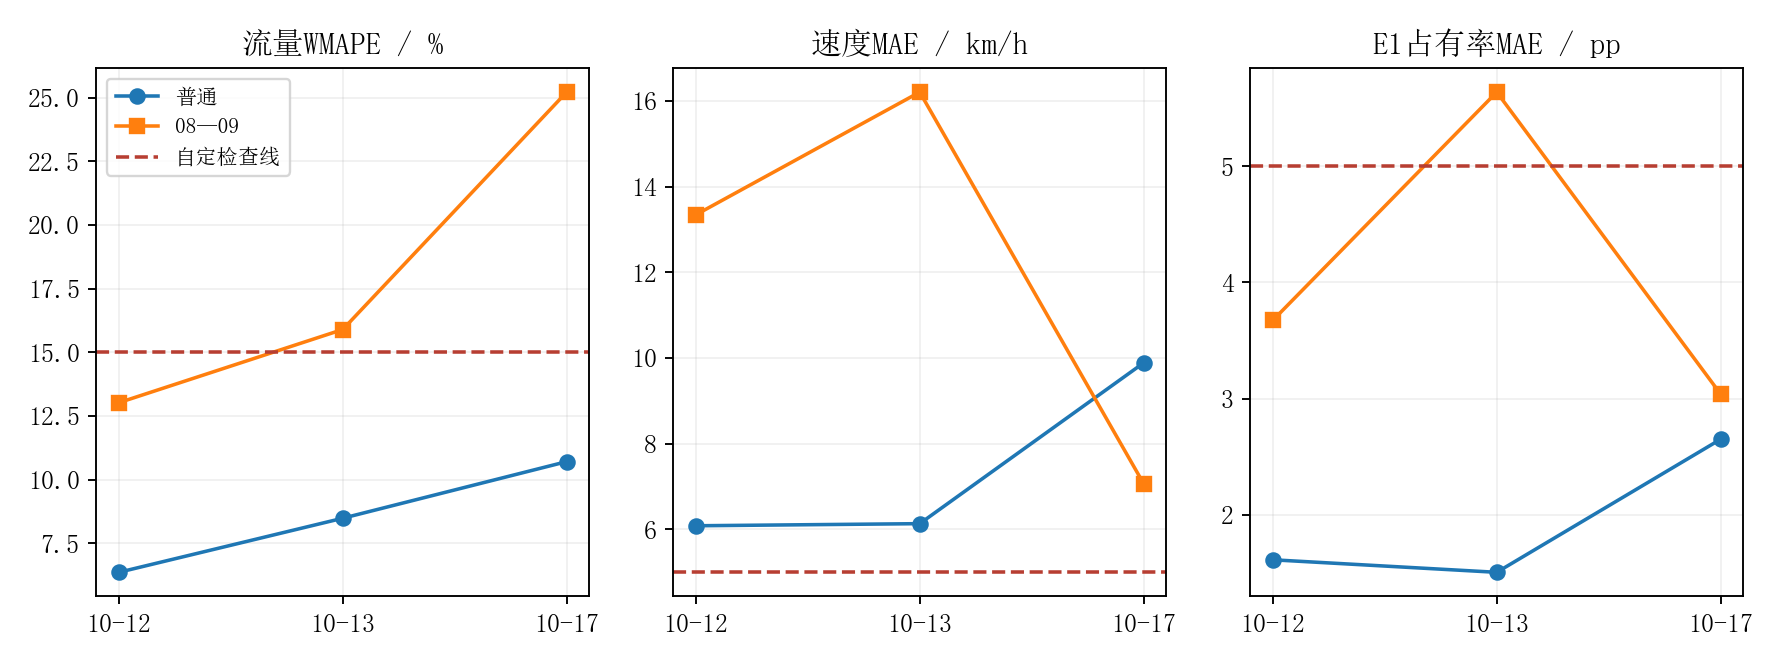
\includegraphics[width=.98\textwidth]{final_figures/crossday.png}
\caption{冻结先验在三日的误差；虚线为项目自定检查线。}
\label{fig:holdout}\end{figure}
表\ref{tab:holdout}及图\ref{fig:holdout}表明流量吻合并不保证速度和拥堵吻合。12、13日早间分别存在2、5个合格低速站窗，先验与滚动均未复现；17日普通时段的1个低速站窗也被漏报，早间没有合格低速站窗。36次联合检查全部失败，滚动更新未形成稳定精度改进。因此只能确认工程功能及已声明范围的迁移运行，不能声称真实高峰已复现。

\subsection{有限联合校准及问题一结论}
为检验剩余可用数据是否支持替换基准，预先限定12个组合，只使用15日训练数据与单一种子，改变入口正则、背景输入、名义供给及一组跟驰时间间隔。评分为流量误差/15、速度误差/5、占有率误差/5、低速漏报比例与错报比例之和，并限制单项退化；要求至少10\%改进后才可读取14日。无观测低速时相应项按预定规则处理，评分用于选择候选，不是现实误差概率。

原评分4.8459，最小评分4.5162，仅改进6.80\%且流量退化，无候选满足采用线。强限流可复现低速5/5，但流量误差25.37\%、占有率误差16.06个百分点，不能按低速单项挑选。14日未打开，未将已看过日期反复调参后称为新验证。
\begin{figure}[H]\centering
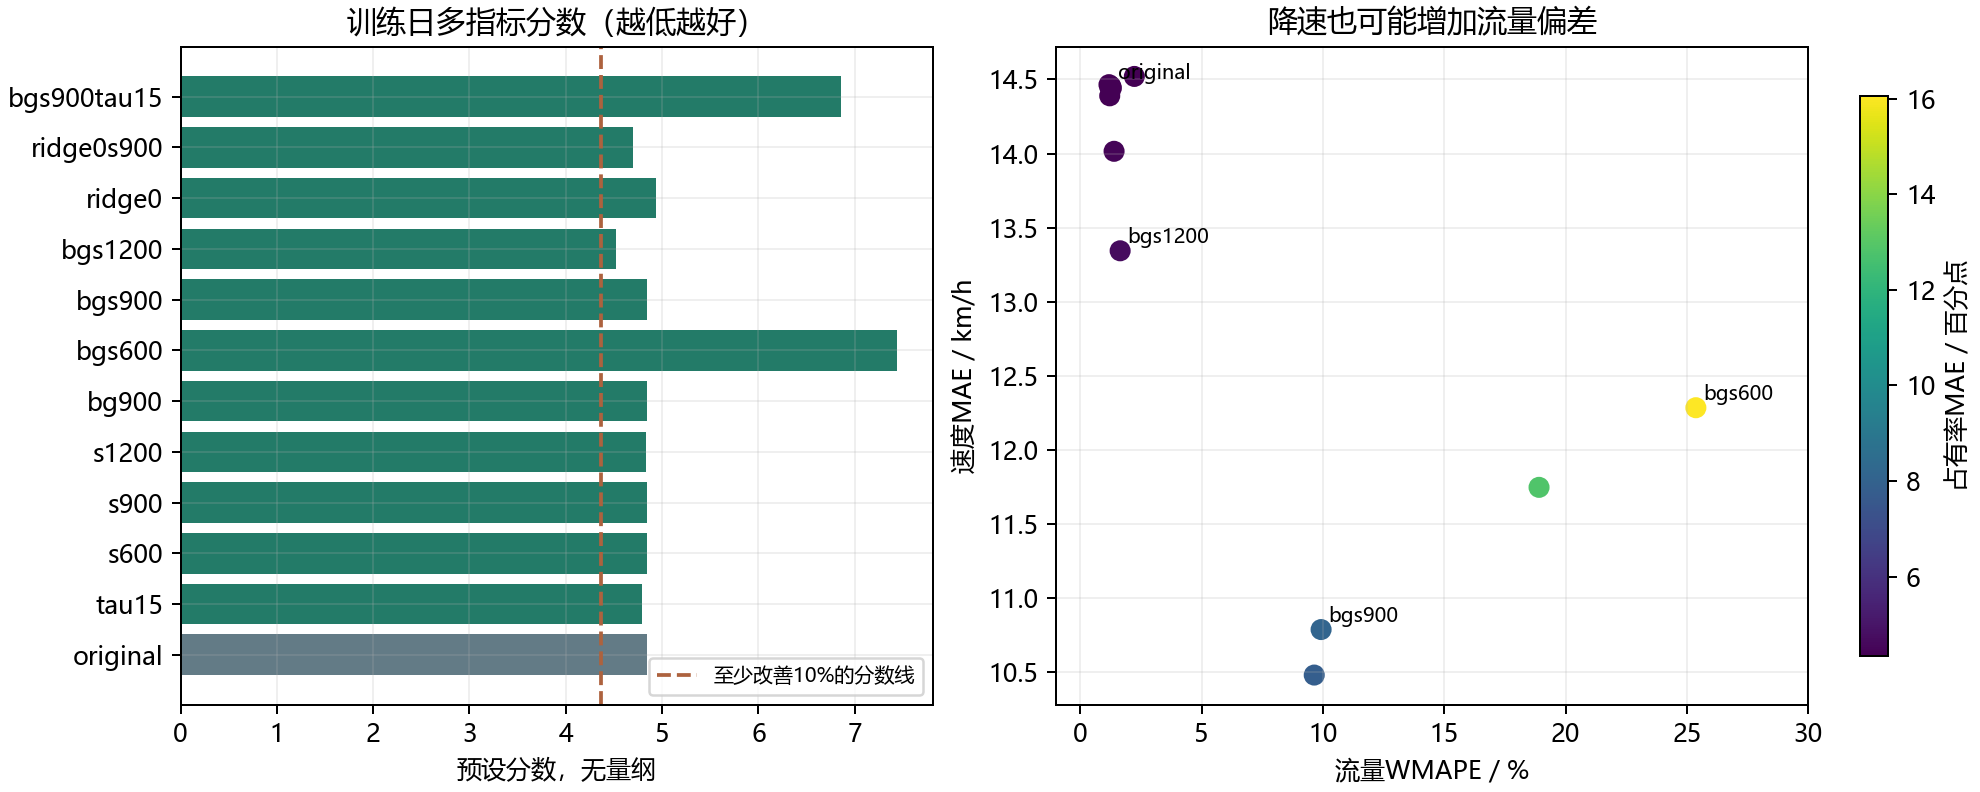
\includegraphics[width=.96\textwidth]{final_figures/calibration.png}
\caption{12个训练组合的误差权衡。未达到采用线，保留原模型。}
\label{fig:calibration}\end{figure}
图\ref{fig:calibration}支持停止本轮有限候选搜索，不证明全局最优。问题一已完成官方数据提取、平行空间、封装系统和泛化试验；真实交通多指标精度仍未达到自定要求。


\section{问题二：条件入口治理A与拥堵实验}
\subsection{结构、实践背景与数据条件：对应二1、二2}
\aicredit
在98条外部边的基准上，于两处支路汇入前设置拟议放行设施，保留原主线和汇入优先关系。治理的作用是调整侧向注入时刻，以降低主线蓄积；付出的代价可能是侧路和入口外等待。三路背景合计900辆/小时、参照下游名义供给900辆/小时及设施参数都是设计值，并非实测路口配时或真实容量。

7种条件分别为参照、核心需求乘0.8/1.2、末端分流比例向侧出/直行移动0.15、供给600/1200辆每小时。分流变化受可替换车辆、相同路径前缀和通行权限约束，实际改变量另存；不声称每辆车均改变0.15。每条件使用20261121—23三个新种子，两策略同网络、同设施、同车辆ID/出发计划/路径/车型、同供给。全绿参照只令拟议入口设施全绿，不表示研究域所有信号全绿。

\subsection{改进平行空间及治理A：对应二3}
占有率控制前进行单车量纲试验：5米车停在93.6米车道时，道路及车道TraCI返回0.0534188，需乘100成为5.34188\%。E1返回及XML为100\%，不能再乘100。道路空间占有率是车辆长度占道路空间的比例，E1是检测断面的时间占用，二者物理定义也不同。此处以本机SUMO 1.27.1实测接口为准，不把修复误用到E1精度指标。

记$o_k$为上一30秒模拟道路空间占有率的百分数，$h_k,l_k$为连续高、低占有率周期数，$a_k$为反馈启用状态，$z_k$为排队保护锁定状态。$o_k\ge18\%$连续2次启用，$o_k\le12\%$连续2次退出。排队数除以假定容纳量达到0.6时锁定全绿，低于0.4解除；锁定优先于启用。未启用与预热均全绿。滞回避免在单阈值附近反复切换，不保证收益。

启用后名义放行率更新为
\begin{equation}
r_{k+1}=\operatorname{clip}\{r_k+30(15-o_k),120,r_{\max}\},\qquad
r_{\max}\in\{1200,1800\}\ {\rm veh/h}.
\label{eq:feedback}
\end{equation}
式\eqref{eq:feedback}中的增益单位为辆每小时每百分点，目标15\%均为设计参数。两设施初始率300/600辆每小时，2车道饱和率按每车道1800辆每小时、启动损失2秒假设，绿灯为$\min(26.5,30r/(1800n)+2)$秒、黄灯3秒。空间容纳量以车道长度除7.5米拥挤间距估算，约199.02/386.18辆。0.6/0.4条件优先于底层遗留0.8放行分支，不能把0.8当最终保护启用线。观测来自模拟传感器，非官方数据直接控制现实信号。

理论上，局部蓄积满足$N_{k+1}-N_k=Q_{\rm in}-Q_{\rm out}$，抑制汇入可能降低下游蓄积；但侧向分流同样影响断面流量，且等待可转移到入口外。因此必须核算全体普通车辆，不能只凭主线速度上升认定治理有效。

\subsection{评价时窗与完整车辆成本：对应二4}
设$p_i,a_i,b_i$为计划出发、实际入网与到达时刻，未完成令$b_i=+\infty$。普通交通在共同评价时窗$[L,H]$中的经历量为
\begin{equation}
C(L,H)=\frac1{3600}\sum_{i\in\mathcal A_{\rm ordinary}}
\max\{0,\min(b_i,H)-\max(p_i,L)\}.
\label{eq:cost}
\end{equation}
式\eqref{eq:cost}从计划出发计入入口外等待，包含预热剩余、待发及未完成。治理$[L,H]=[300,3900]$对应08—09；清空继续至5700秒，末期未完成另报。种子$j$的配对变化为$\delta_j=100(C_{A,j}/C_{{\rm free},j}-1)$，条件均值是三个$\delta_j$的均值。七条件没有现实概率，不计算其现实期望收益。

\begin{table}[H]\centering
\caption{正确单位治理A的21组配对；负号表示总经历量降低}\label{tab:governance}
\begin{tabularx}{\textwidth}{Yrrr}\toprule
条件 & 平均变化\% & 最差变化\% & 恶化组/3\\\midrule
参照 & −5.16 & −2.77 & 0\\
核心需求0.8倍 & −0.23 & +0.06 & 2\\
核心需求1.2倍 & −22.79 & −21.32 & 0\\
增加侧向退出 & +0.40 & +1.30 & 2\\
增加直行 & −4.93 & −1.74 & 0\\
名义供给600 & −14.77 & −12.54 & 0\\
名义供给1200 & −0.56 & −0.19 & 0\\\bottomrule
\end{tabularx}\end{table}
表\ref{tab:governance}中17/21组改善、4/21组恶化；最差增加1.2986\%。需求较大或供给较小条件下的改善更明显，但条件不是按现实发生概率抽样，不可据此建议现实直接部署。

\begin{figure}[H]\centering
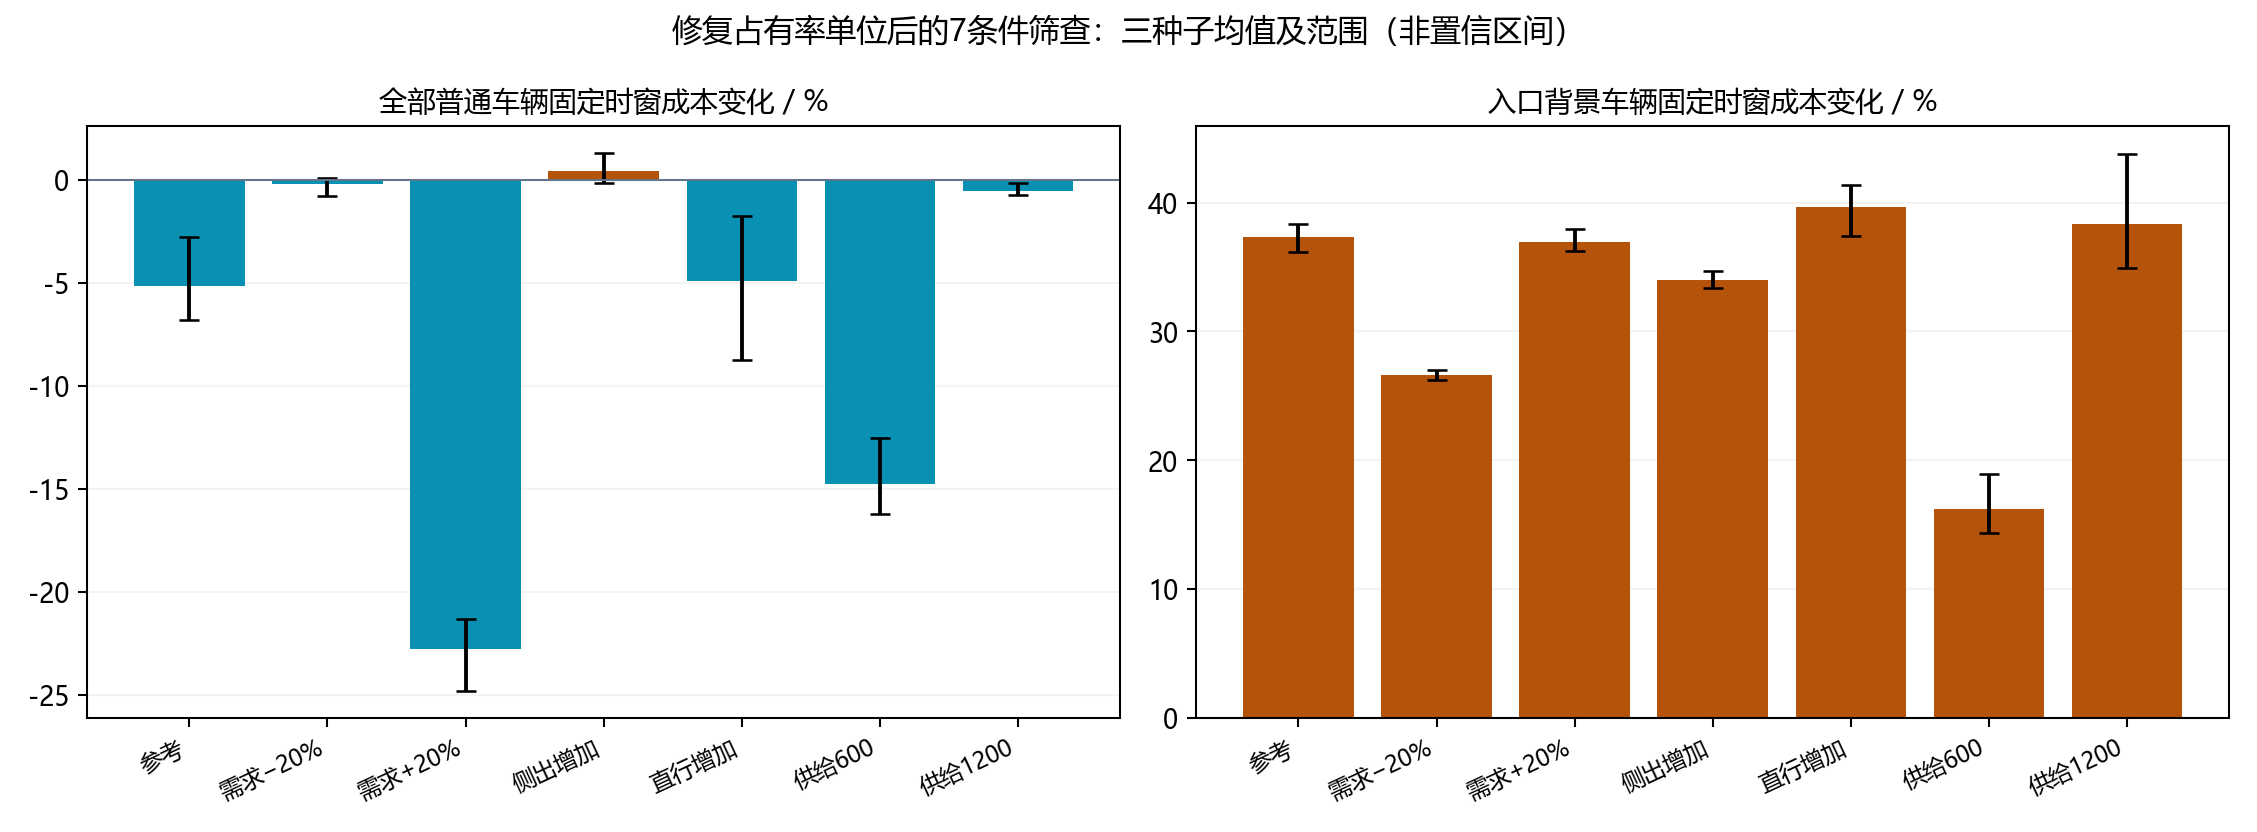
\includegraphics[width=.98\textwidth]{final_figures/governance.png}
\caption{同输入治理A的总成本与背景代价；不省略恶化配对。}
\label{fig:governance}\end{figure}
图\ref{fig:governance}中背景车21/21组经历量增加，范围14.34\%—43.77\%；6/21组共同清空末未完成增加。两个入口的排队保护均未触发，不能声称保护效果已得到验证。42次仿真均零瞬移、零碰撞、守恒差零，控制日志按状态转移和绿灯公式逐项复算；这些是实现核验，不替代现实有效性。

\subsection{等待保护候选及稳定收益边界}
考虑原控制可能让背景车长期等待，预先定义120秒与240秒等待保护，使用原开发种子21、22各7条件共28次。保护代理包括已到计划出发但未入网的等待，以及进路停车和入口延迟；它不是单车最终等待的严格上限。TraCI在步末报告插入，较XML步起点有0.5秒差，保护代理保守多计至多0.5秒，正式成本仍用XML实际时刻。

\begin{table}[H]\centering
\caption{等待保护相对保留方案的开发结果，全部未采用}\label{tab:waiting}
\begin{tabularx}{\textwidth}{Yrrr}\toprule
候选 & 背景选型均值\% & 最差总成本\% & 最差条件均值未完成增量\\\midrule
120秒 & −23.53 & +28.04 & +298.0辆\\
240秒 & −20.23 & +21.65 & +251.5辆\\\bottomrule
\end{tabularx}\end{table}
表\ref{tab:waiting}说明减轻背景等待会牺牲主线总成本和末期完成量。两候选均未达预设采用线，未进入新种子复验，不能把开发平均改善当作新验证。保留修复后的原治理A，不宣称其已解决公平性或有普遍稳定收益。

\subsection{与基准比较及问题二结论：对应二5}
问题一用于检验观测约束下基准精度；本问用完全同输入的拟议入口全绿作参照，从而隔离控制作用。不同日期、车辆数和网络的总耗时不直接相除为治理收益。控制能够在若干设计拥堵条件下降低总经历量，但所有背景配对受损，部分条件总成本增加。缺少真实转向、配时与初态时，结论限于设计实验；本轮候选未提供可靠替换证据。


\section{问题三：道路应急治理B与保障协同}
\subsection{孪生结构、实践背景及数据条件：对应三1、三2}
\aicredit
在基准上增加任务路线及信号相关道路，共125条外部边。为避免将未核实的医院专用入口作为必要前提，任务改为从道路1433971795插入、到1095134811下游端到达，10条外部边长1063.1米，不含内部连接。起终点与官方中心线最近距离约2.35/1.46米，仅支持地理接近，不证实应急驻点、准入或停车许可。

08:30—08:45对道路771547540的单车道施加3米每秒作业限速，之后恢复；08:35调度一辆合成应急代理，09:30共同截止。供给、背景车辆及拟议设施与治理A体系一致。180秒为项目设计诊断线，不是官方救援标准；模型未包含真实基地准备、停车、现场救治、病人装载或医院交接。

\subsection{改进平行空间及协同规则：对应三3}
任务代理增加调度时刻、固定路径、任务状态及预计到达，事件代理保存开始/结束和恢复限速。协同控制每2秒读取当时状态，稀疏让行只考虑60米内最近前车，双方速度不超过5米每秒。目标车道须满足权限、下一路段和约120米路径连续性，前后空位至少为3米加1.5秒速度余量，并通过SUMO换道检查；距路口25米内不请求，同车同路段至多一次，另设30秒冷却。换道通过TraCI执行\cite{vehicle}，保留全部默认安全模式。

已绿延长按距停止线距离$/\max(v,3)$估计到达，另加2秒余量，最多延长10秒；不跳红、不改变相容状态\cite{signal}。低速时该到达估计可能偏乐观。请求后4秒检查车辆位置，离开原路段记无法判断；动作确认不自动等于任务因果收益。

采用20261125—27三个新种子，比较治理A但无专门协同、A加稀疏让行、A加让行和延绿，9次同输入运行。看到这9次结果后，再预先固定补充全绿参照的3种子及规则，保留全部3次。后者是事后诊断，不能追称盲测。额外策略差异均在相同125边、任务、事件和车辆下核算。

\subsection{步长对应、任务与普通交通结果：对应三4}
图\ref{fig:physical}取预设首种子的A加协同运行，按式\eqref{eq:clock}对齐物理时刻；仿真结果由系统状态文件输出，不能以视频播放秒当作案例物理秒。
\begin{figure}[H]\centering
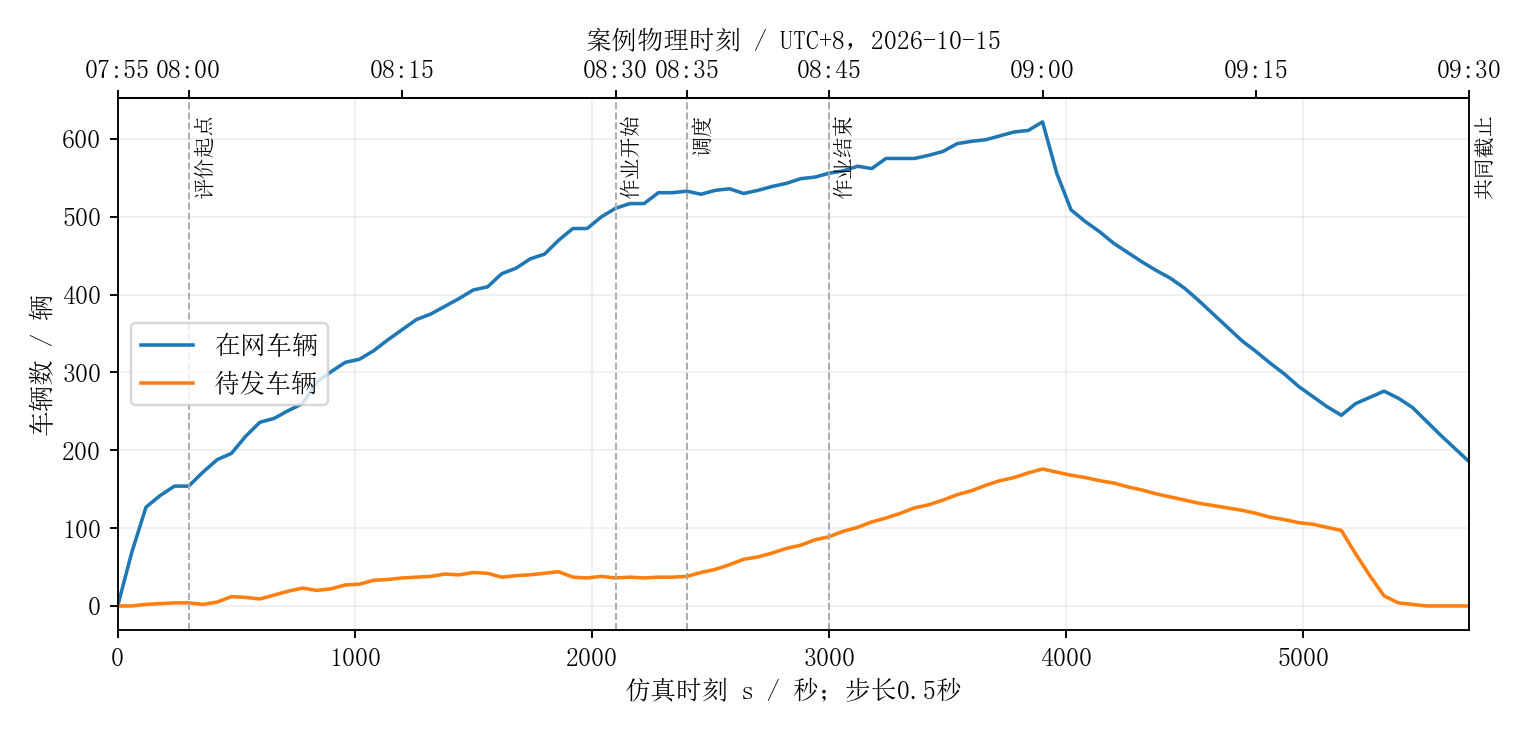
\includegraphics[width=.98\textwidth]{final_figures/physical_time.png}
\caption{0.5秒仿真步与物理时空对应；显示在网、入口外待发及事件时刻。}
\label{fig:physical}\end{figure}
任务评价从计划调度到到达；若未到达，应保留截止经历下界。普通交通排除应急车，按式\eqref{eq:cost}统计08—09:30全体普通车经历量，与问题二08—09口径区分。

\begin{table}[H]\centering
\caption{道路任务三组结果；A加专门协同与A数值完全相同}\label{tab:tasks}
\begin{tabularx}{\textwidth}{Yrrrr}\toprule
种子 & 全绿任务s & A任务s & 普通成本变化\% & 背景变化\%\\\midrule
20261125 & 642.5 & 91.0 & −5.18 & +68.76\\
20261126 & 1164.5 & 124.5 & −6.49 & +65.81\\
20261127 & 1934.0 & 79.0 & −10.15 & +66.14\\\bottomrule
\end{tabularx}\end{table}
\begin{figure}[H]\centering
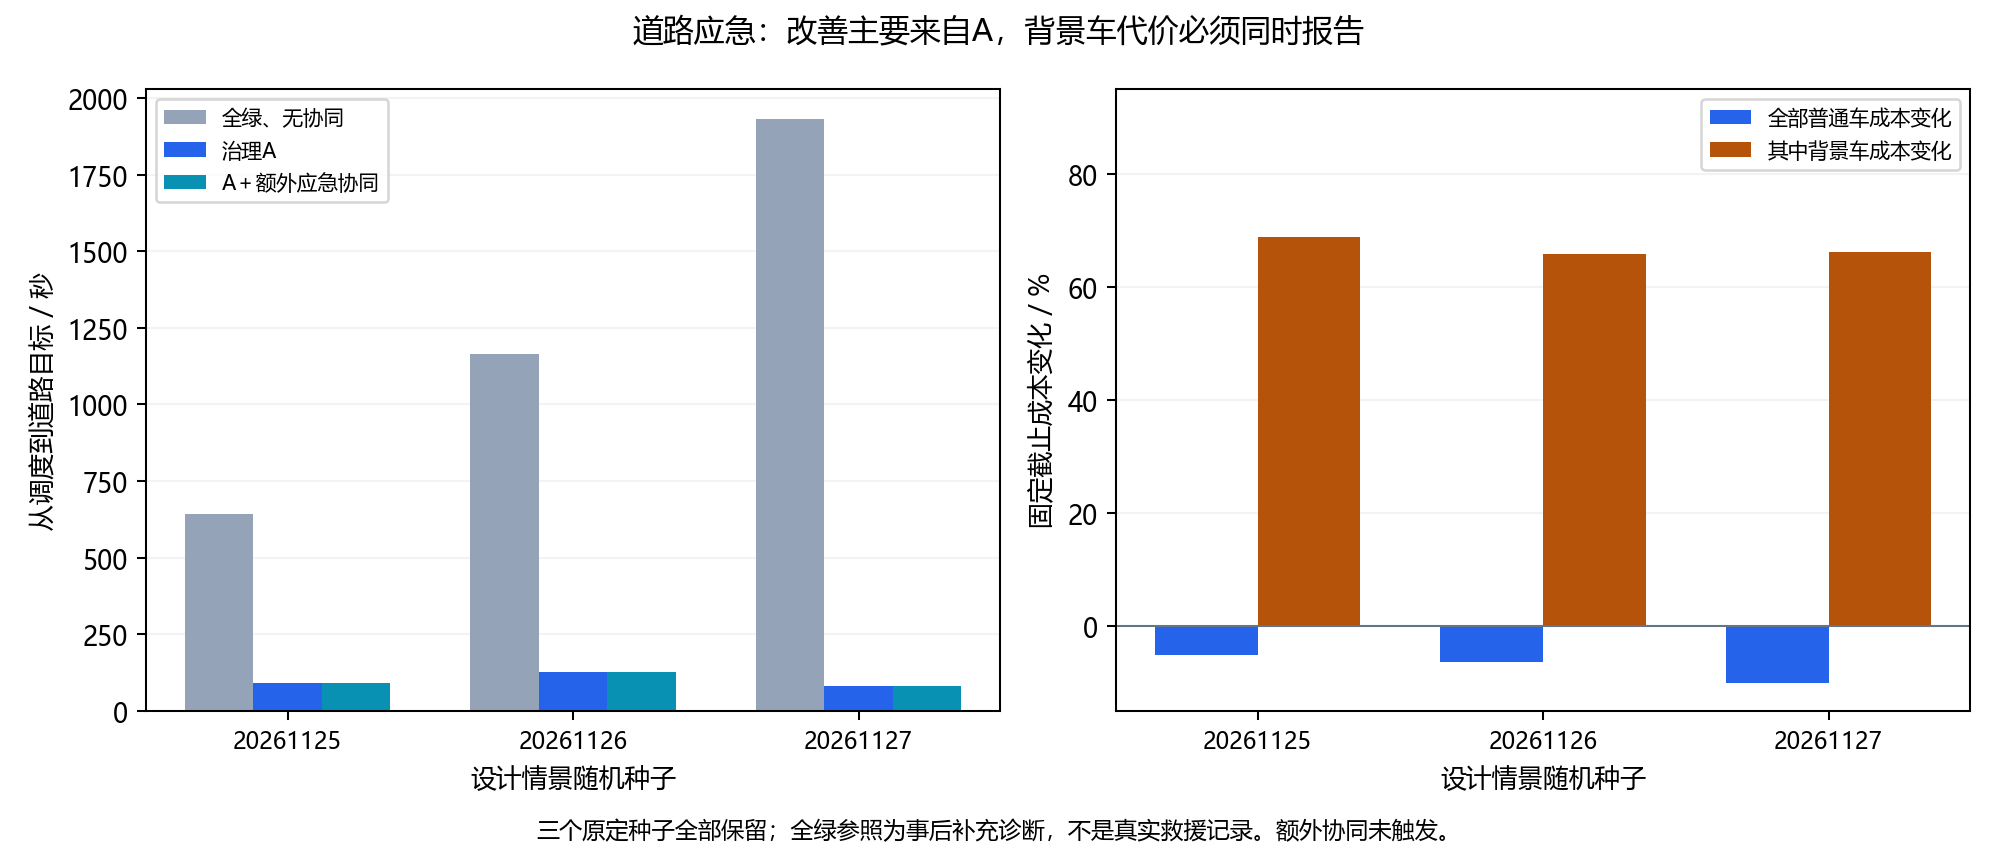
\includegraphics[width=.98\textwidth]{final_figures/road_task.png}
\caption{同道路任务下的全绿、治理A及A加协同结果；全绿为补充诊断。}
\label{fig:task}\end{figure}
表\ref{tab:tasks}与图\ref{fig:task}中12次均到达，A背景下任务达到180秒设计线。全绿到A的任务差异很大，但不能归功于额外让行或延绿：两类请求均为0，A加协同完全未增益。普通成本下降的同时，普通未完成全绿到A分别177→185、192→225、212→225辆，背景成本明显上升，不能称全部交通改善。

\subsection{轻中重作业扩展及无触发解释}
进一步在冻结原道路任务下，将单车道作业限速设为6/3/1米每秒，使用新种子20261221—23，每级比较全绿、A及A加协同，共27次。全部任务到达；让行请求0、延绿0，额外协同相对A的任务和普通成本变化均为0。各级在本批得到相同关键结果，说明设置的作业强度没有在这些输入和轨迹中形成可辨识的额外协同需求，不能解释为已证明策略不受事件严重程度影响。

规则有分支且程序可运行，不等于已验证其有效作用。若以后取得真实任务、初始排队、信号和阻塞几何，应重新冻结可触发协同的独立场景并验证，不能为做出收益而继续挑选当前种子。

\subsection{与前项比较及问题三结论：对应三5}
应急任务的A到A加协同是额外治理B的增量比较；同场景全绿到A是入口治理在道路任务中的条件性影响。问题二和本问网络、事件及评价时窗不同，不将两个章节成本直接计算为改善率。现有证据表明道路任务在设计参照下能够到达，入口治理改变了拥堵及任务耗时分布，但代价转移到背景交通，未证明额外应急协同的新增收益或现实救援有效性。


\section{模型评价、证据边界与复现}
系统在同一封装中实现官方数据提取、时间身份保存、非唯一需求估计、代理交互、控制事件、物理时间输出及离线回放。固定车辆清单与共同截止成本使入口外等待和未完成留在结果中，便于判断收益是否只是等待转移。模型数值、道路单位、控制决策和车辆守恒均有程序核验；自动复算由AI辅助完成，不能写成参赛者独立人工核验。

\begin{table}[H]\centering
\caption{成果达到的范围与未证实事项}\label{tab:limits}
\begin{tabularx}{\textwidth}{lYY}\toprule
方面 & 现有证据 & 未达到或仍缺的数据\\\midrule
GIS与观测 & 官方中心线、来源哈希、时间和质量标签 & 9个映射复核标记、部分新镜头接入失败\\
一般交通 & 36次跨日验证、三指标及低速评价 & 真实高峰联合精度未通过，初始队列未知\\
治理A & 21配对、完整成本、7条件压力比较 & 4组恶化、背景全部受损、无普遍稳定收益\\
道路应急 & 12次及27次扩展全到达 & 专门协同零触发，真实派遣/停车/救护门未知\\
连续运行 & 实际一小时、60次HTTP、守恒核算 & 12次均保持、未证明精度或全天候运行\\
有限优化 & 等待28、训练12、应急27次全报告 & 均无合格替换，不证明不存在其他优化\\\bottomrule
\end{tabularx}\end{table}
表\ref{tab:limits}界定了“能运行”“设计情景有效”和“现实有效”的差别。缺少真实转向、配时、供给和排队初态时，再增加复杂优化器不能自动补出缺失信息。本轮有限候选已按停止规则收口，保留正确单位原方案，后续优先收集可独立检验的数据。

开发累计349次包括历史错误单位、失败及输入诊断，不是349个真实独立样本，也不是349次正确模型验证。历史结果只用于追溯，不与本版治理收益混合。支撑保留逐运行清单、完整车辆结果、输入、全部配对与失败汇总，具体归档数量以支撑清单为准；视频的另行重演不计入新策略实验。

\file{python reproduce.py verify --output checks}仅用Python标准库，检查哈希并复算全部归档普通成本、背景成本及未完成；重演还需Python依赖与SUMO 1.27.1。当前控制的冻结输入可由\file{run}子命令重演，动态计划按已实现车辆计划重演，不重新请求旧HTTP，也不保证动态加入与静态重演完全同轨迹。原实时接口入口另保留，联网重新采集不等于重现旧观测。独立解压验收、文件大小及哈希记录在交付清单，未完成的人工事实不由脚本代填。
\begin{thebibliography}{99}
\raggedright
\bibitem{gis} 香港特别行政区运输署. 第二代道路网络数据文件目录. \url{https://static.data.gov.hk/td/road-network-v2/dataspec/file_list.csv}, 访问日期：2026-10-18.
\bibitem{traffic} 香港特别行政区运输署. Data Specification for Traffic Data of Strategic / Major Roads, Last Update 30 November 2022. \url{https://static.data.gov.hk/td/traffic-data-strategic-major-roads/dataspec/dataspec-traffic-data-strategic-major-roads.pdf}, 访问日期：2026-10-18.
\bibitem{archive} 香港政府资料一线通. Historical Archive API: list-file-versions. \url{https://app.data.gov.hk/v1/historical-archive/list-file-versions}, 查询对象rawSpeedVol-all.xml、日期2026-10-12、13、17；访问日期：2026-10-18.
\bibitem{hospital} 香港医院管理局. Hospital Authority Open Data: Hospitals. \url{https://www.ha.org.hk/opendata/facility-hosp.json}, 访问日期：2026-10-18.
\bibitem{osm} OpenStreetMap Foundation. Licence. \url{https://osmfoundation.org/wiki/Licence}, 访问日期：2026-10-18.
\bibitem{sumo} Eclipse SUMO. Basic Definition. \url{https://sumo.dlr.de/docs/Simulation/Basic_Definition.html}, 访问日期：2026-10-18；实际运行版本1.27.1.
\bibitem{traci} Eclipse SUMO. TraCI. \url{https://sumo.dlr.de/docs/TraCI/index.html}, 访问日期：2026-10-18.
\bibitem{krauss} Eclipse SUMO. Car-Following-Models. \url{https://sumo.dlr.de/docs/Car-Following-Models/index.html}, 访问日期：2026-10-18.
\bibitem{scipy} SciPy Developers. scipy.optimize.lsq\_linear. \url{https://docs.scipy.org/doc/scipy/reference/generated/scipy.optimize.lsq_linear.html}, 访问日期：2026-10-18. 在线文档版本不代指本机安装版本.
\bibitem{aivas} 香港特别行政区运输署. Traffic Data from AI Video Analytics System of CCTVs, Data Specification. \url{https://www.td.gov.hk/datagovhk_td/traffic-data-aivas/resources/traffic_data_from_ai_video_analytics_system_of_cctvs_dataspec.pdf}, 访问日期：2026-10-18.
\bibitem{tad} 香港特别行政区运输署. Traffic Aids Drawings (2nd generation). \url{https://data.gov.hk/en-data/dataset/hk-td-tis_16-traffic-aids-drawings-v2}, 实际取得DTAD\_TS\_ABV\_ANNO\_PT及DTAD\_TRAFFIC\_LIGHT\_PT的GML；访问日期：2026-10-18.
\bibitem{hospitalmap} 香港医院管理局伊利沙伯医院. Maps and Directions; Transportation. \url{https://www3.ha.org.hk/qeh/eng/patients/maps-directions.htm}; \url{https://www3.ha.org.hk/qeh/eng/patients/transportation.htm}, 访问日期：2026-10-18.
\bibitem{vehicle} Eclipse SUMO. Change Vehicle State. \url{https://sumo.dlr.de/docs/TraCI/Change_Vehicle_State.html}, 访问日期：2026-10-18.
\bibitem{signal} Eclipse SUMO. Traffic Lights. \url{https://sumo.dlr.de/docs/Simulation/Traffic_Lights.html}, 访问日期：2026-10-18.
\bibitem{ai} OpenAI. Codex，具体模型版本及发布日期【待补充】. OpenAI，实际使用记录见支撑材料工作稿，日期2026-10-17—18. 本条为待完善的工具披露，不作为方法依据.
\end{thebibliography}


\section*{AI工具使用说明}
\addcontentsline{toc}{section}{AI工具使用说明}
本项目使用OpenAI Codex\cite{ai}辅助赛题解释与数据来源查询、数据清洗和估计、模型设计、仿真程序实现与调试、实验及有限参数搜索、自动结果核验、图表、管理页面、论文撰写和演示视频。这些属于实质性工作。各技术章节已明确标注AI贡献，程序注释与支撑中的《AI工具使用详情.pdf》同步说明。

参赛者此前明确表示尚未完成人工修改和结果复核；截至本版生成，未获得完成这些工作的确认。具体历史模型、版本发布日期、其他工具及完整真实交互仍待补充，不虚构人工核验。现有文件是技术定稿待本人复核版，AI披露材料尚不足以直接提交。是否满足本比赛核心建模、仿真实现与分析由队员独立完成的规定，须由实际工作和当年正式规则判断，不能因披露或自动检查而认定合规。

\appendix
\clearpage
\section{支撑材料列表与复现入口}
\begin{longtable}{p{.27\textwidth}p{.65\textwidth}}
\toprule 文件 & 内容与用途\\\midrule\endhead
\file{README.md} & 环境、包结构、命令、未通过指标及复核缺项。\\
\file{requirements.txt} & Python依赖；SUMO另行安装。\\
\file{support.json} & 逐运行索引、输入/结果/数据来源、SHA256与复算目标。\\
\file{reproduce.py} & 标准库完整性及全部车辆成本复算、按运行ID提取与重演。\\
\file{payload.xz} & 按内容去重的源程序、片区数据、仿真输入与完整车辆结果。\\
\file{AI工具使用详情.pdf}及Word & 已知真实用途、可见提示摘要、采纳情况和待补信息。\\
\file{论文源码/} & 本文TeX及实际使用图表；不分发字体和第三方软件。\\\bottomrule
\end{longtable}
\file{payload.xz}由\file{support.json}索引，可用\file{extract}命令提取为常规目录。其中\file{source/}保存应用与冻结源码；\file{data/}保存实际使用的区域GIS、观测、质量与来源；\file{runs/}保存输入、结果、指令及逐车时刻；\file{reports/}保留全部配对、失败、旧单位版本及修复后的说明。车辆结果按完整清单行序无损关联，不删除待发及未完成。XML只去掉本机生成注释，JSON匿名化路径，原始与归一化哈希分别保存。

完整全港GIS和全港原始归档不重复分发，实际使用的区域记录、来源URL及原件哈希保留；重复图表与逐步界面缓存留在开发工作区。视频按规则单独提交。承诺书、密钥、姓名学校及第三方二进制不进入匿名包。准备材料未代替本人签字或实际上传。
\end{document}
